\documentclass{llncs}
\usepackage{graphicx}
\graphicspath{ {images/} }


\title{\textbf{Random Forest vs Logistic Regression for Binary Classification}}
\author{Kaitlin Kirasich, Trace Smith, and Bivin Sadler, PhD$^1$}
\institute{$^1$Master of Science in Data Science \\ Southern Methodist University \\ Dallas, Texas USA \\
\email{kkirasich@.smu.edu,traces@smu.edu,bsadler@smu.edu}}

\begin{document}
\maketitle

\begin{abstract} 
Selecting a learning algorithm to implement for a particular application on the basis of performance still remains an ad-hoc process using fundamental benchmarks such as evaluating a classifier’s overall loss function, area under the curve (AUC) score, specificity, and sensitivity values. This work is aimed at addressing the difficulty of model selection by evaluating the overall classification performance between random forest and logistic regression for datasets comprised of various underlying structures. A model evaluation tool was developed in R for simulating a variety of datasets types in order to evaluate performance metrics such as true positive rate, false positive rate, and accuracy under specific conditions. Our findings indicate that when increasing the variance in the explanatory and noise variables, logistic regression consistently performed with a higher overall accuracy as compared to random forest.  However, the true positive rate for random forest was higher than logistic regression and yielded a higher false positive rate. In all cases a paired two sample t-test indicates there is enough evidence to suggest the false positive rate for random forest is statistically different than logistic regression. The model evaluation application developed in this work is a proxy for answering other intruiguing questions related to model performance under various treaments. 

\end{abstract}

\section{Introduction}

\section{Motivation}

\section{Data Set}


\begin{figure}
\centering
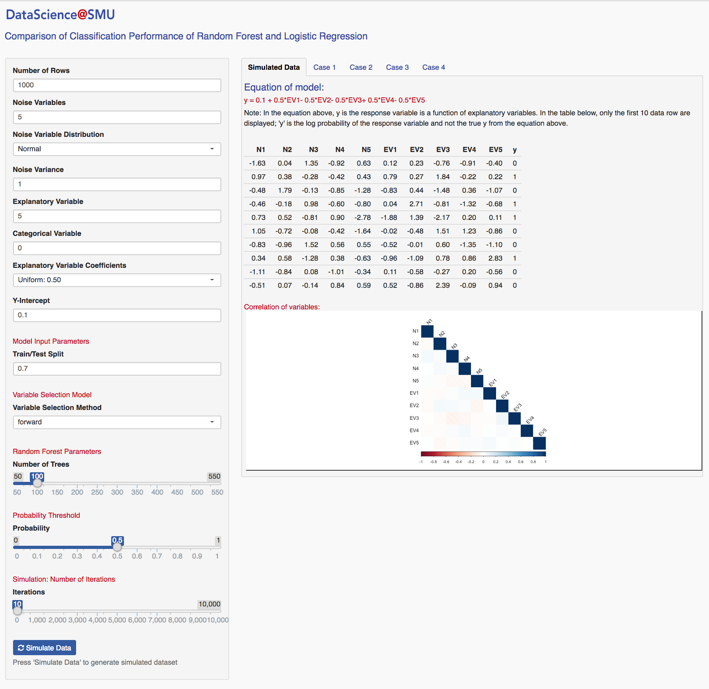
\includegraphics{rshiny.png}
\caption{R Shinny Application - Data Simulator}
\end{figure}


\section{Methods and Experiments}

The two machine learning algorithms studied in this work consisted of random forest and logistic regression. Both models have been implemented in a wide range of domains for predicting class labels and are not only known for their success, but simplicity to implement and relatively straightforward to interpet. A overview of the two models are provided in the following sections.

\subsection{Random Forest}

Random forest is an ensemble based learner which is comprised of 'n' collection of de-correlated trees (Hastie, 2009). Built off the idea of bootstrap aggregation which with a method for resampling with replacement in order to reduce variance, random forest uses multiple trees to average (regression) or computes majority votes (classification) in the terminal leaf nodes when making a prediction. Decision trees themselves are prone to overfitting noise in a training set which ultimately leads to results with high variance. In other words, this means the model could accurately predict the same data it was trained on but may not possess the same performance on datasets without the similar patterns and variations in the training set. As previously stated, random forest solves this overfitting of data by averaging multiple decision trees trained on different parts of the training set. 

\subsection{Logistic Regression}

Linear models are composed of one or multiple independent variables that describes a relationship to a dependent response variable. Mapping qualitative or quantitative input features to a target variable that is attempted to being predicted such as financial, biological, or sociological data is known as supervised learning in machine learning terminology if the labels are known.  One of the most common utilized linear statistical models for discriminant analysis is logistic Regression.

\begin{equation}
\pi_{i} = \beta_{0} + \beta_{1}X_{1} + .....\beta_{n}X_{n}
\end{equation}

Simplicity and interoperability of logistic Regression can occasionally lead to outperforming other sophisticated nonlinear models such as ensemble learners or support vector machines. However, in the event the response variable is drawn from a small sample size, then linear regression models become insufficient and performs poorly for binary responses A number of learning algorithms could be applied to modeling binary classification data types, however the focal point of this work is to examine one linear model, logistic regression. 
 
Unlike the response variable for Linear Regression which is quantitative, the target variable for logistic regression is the posterior probability of being classified in the ith group of a binary or multi-class response (Hastie, 2009). Logistic regression makes several assumptions such as independence, responses (logits) at every level of a subpopulation of the explanatory variable are normally distributed, and constant variance between the responses and all values of the explanatory variable. Intuitively, a transformation to the response variable is applied to yield a continuous probability distribution over the output classes bounded between 0 and 1; this transformation is called to “logistic” or “sigmoid” function where ‘z’ corresponds to log odds divided by the logit (Ng, 2008).

\begin{equation}
\sigma(Z) = \frac{1}{1+\exp^{-z}}
\end{equation}


\begin{figure}
\centering
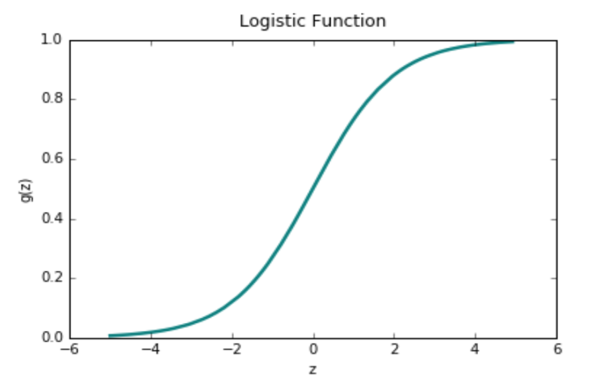
\includegraphics[scale=1.0]{sigmoid.png}
\caption{Log of Odds Function}
\end{figure}

For a binary response, the logistic regression model can be expressed by summing over the linear combinations of input features and a corresponding weight plus a bias terms for each instance as shown below in equation (3) and (4).

\begin{equation}
p(y^{(i)} = 1 | x^{(i)},w) = 1-  \frac{1}{1+\exp^{(w^{T}x^{(i)}+b)}}
\end{equation}
\begin{equation}
p(y^{(i)} = 0 | x^{(i)},w) = 1-  \frac{1}{1+\exp^{(w^{T}x^{(i)}+b)}}
\end{equation}


The objective is to find a set of weights such that the negative log likelihood is minimized over the defined training set using optimization techniques such as gradient descent or stochastic gradient descent [3]. Minimizing the negative log likelihood also means maximizing the likelihood or probability the parameter estimate pi of selecting the correct class. The loss function that measures the difference between the ground truth label and the predicted class label is referred to as the cross-entropy. If the prediction is very close to the ground truth label, the loss value will be low. Alternatively, if the prediction is far from the true label, the resulting log loss will be higher.

\begin{equation}
J(\theta) = -\frac{1}{m}\sum p_{i}log(y_{i}) + (1-p_{i})log(1-y_{i})
\end{equation}



\section{Results}




\section{Analysis}



\section{Ethics}



\section{Conclusions}



\end{document}

